%% LyX 2.2.2 created this file.  For more info, see http://www.lyx.org/.
%% Do not edit unless you really know what you are doing.
\documentclass[english]{article}
\usepackage{mathptmx}
\usepackage{graphicx}
\usepackage{helvet}
\usepackage{courier}
\usepackage[T1]{fontenc}
\usepackage[latin9]{inputenc}
\usepackage{geometry}
\geometry{verbose,tmargin=2.5cm,bmargin=2.5cm,lmargin=2.5cm,rmargin=2.5cm,headheight=0cm,headsep=0cm}

\makeatletter
\@ifundefined{date}{}{\date{}}
\makeatother

\usepackage{babel}
\begin{document}

\title{The Programming Assignment Report Instructions\\
CSCE 221}
\maketitle
\begin{enumerate}
\item The description of an assignment problem.\\ \ \\
The purpose of this assignment is to be able to take an input of cities with info on where each city has a flight to another city. From this information, using a graph data structure and BFS, the shortest path from one city to another is determined.
\\
\item The description of data structures and algorithms used to solve the
problem.
\begin{enumerate}
\item Provide definitions of data structures by using Abstract Data Types
(ADTs) \\
\begin{itemize}
  \item \textbf{Linked List}: a sequence of nodes where each node contains a pointer to the  next node in the sequence. Since it is templated, a variety of data types can be passed in.
  \item \textbf{Que:} a linear data structure where operations are performed based on first-in-first-out principle. Since it is templated, a variety of data types can be passed in.
  \item \textbf{String:} a container that holds an array of characters
  \item \textbf{Vector:} a container that can hold a variety of data types. Vector has several built in functions. Also provides bounds error checking.
  \item \textbf{Graph represented by an adjacency list: } in this assignment the graph was implemented as a vector of linked list of edges.
them. 
\end{itemize} \ \\
\item Write about the ADTs implementation in C++.\\ \ \\
\begin{itemize}
  \item \textbf{Linked List}: in this assignment the C++ standard library implementation of a linked list was used. It was used in the adjacency list.
  \item \textbf{Que:} in this assignment the C++ standard library implementation of a que was used. It was used in implementing the BFS.
  \item \textbf{String:} in this assignment the C++ standard library implementation of a string was used
  \item \textbf{Vector:} in this assignment the C++ standard library implementation of a vector was used. Int was used for the ajacency list, container to hold vertices, and container for holding the edges.
  \item \textbf{Graph represented by an adjacency list: } this was used to arrange all the cities and their connections.
\end{itemize} \ \\

\item Describe algorithms used to solve the problem.\\
\begin{itemize}
  \item \textbf{BFS/shortest distance: } A BFS traversal of a graph G visits all the vertices and edges of G, determines whether G is connected, computes the connected components of G, then finds the shortest path once the endpoint is found. This is done by first pushing the starting vertex to the queue. Also push this vertex to the visited vector with a NULL parent. While the queue is not empty, pop the queue. if this popped queue is the vertex being searched for, go to the vector and traverse up from the found vertex to its parents until the starting vertex is found, that is the shortest path. Else, go to the next level of the graph and enqueue each vertex in that level as well as pushing back each vertex and its parent to the visited vector. 
  \item \textbf{BuildGraph: } read in the first line to determine the number of vertices and number of edges. Iterate through the remaining lines to determine  what vertices are connected to $v_{i - 1}$.
  \item \textbf{Determine Partitioning: } this algorithm purpose is to determine the possibility
of partition the cities into two groups such that there is no edge between two vertices in each group. Iterate through each vertex. Check if the given vertex is not in group a or group b, if so add to group a. Check if vertex is in group a but not group b,  
\end{itemize}

\item Analyze the algorithms according to assignment requirements. \\
\begin{itemize}
  \item \textbf{BFS/shortest distance: } $O(V+E)$
  \item \textbf{BuildGraph: } $O(V+E)$
  \item \textbf{Determine Partitioning: } $O(V+E)$
\end{itemize}
\end{enumerate}

\item A user guide description how to navigate your program with the instructions
how to: 
\begin{enumerate}
\item compile the program: specify the directory and file names, etc.\\
'g++ *.cpp -o run.out' in root directory I submitted 
\item run the program: specify the name of an executable file. \\
./run.out \{file-name\}
\end{enumerate}
\item Specifications and description of input and output formats and files 
\begin{enumerate}
\item The type of files: keyboard, text files, etc (if applicable). \\ \ \\
Input file containing the cities and the connections between the cities \\
\item A file input format: when a program requires a sequence of input items,
specify the number of items per line or a line termination. Provide
a sample of a required input format. \\ \ \\
Example input, \\
7 6 \\
1 2 -1 \\
0 3 4 -1 \\
0 5 6 -1 \\
1 -1 \\
1 -1 \\
2 -1 \\
2 -1
\\
\item Discuss possible cases when your program could crash because of incorrect
input (a wrong file name, strings instead of a number, or such cases
when the program expects 10 items to read and it finds only 9.)\\ \ \\
The program will crash if the input first line does not specify the correct number of vertixes and edges.
\end{enumerate}
\item Test your program for correctness using valid, invalid, and random
inputs (e.g., insertion of an item at the beginning, at the end, or
at a random place into a sorted vector). Include evidence of your
testing, such as an output file or screen shots with an input and
the corresponding output. \\ \ \\
With the following input, \\
4 4 \\
1 3 -1 \\
2 0 -1 \\
1 3 -1 \\
0 2 -1 \\
Results in the following output
\begin{figure}[h]
  \begin{center}
    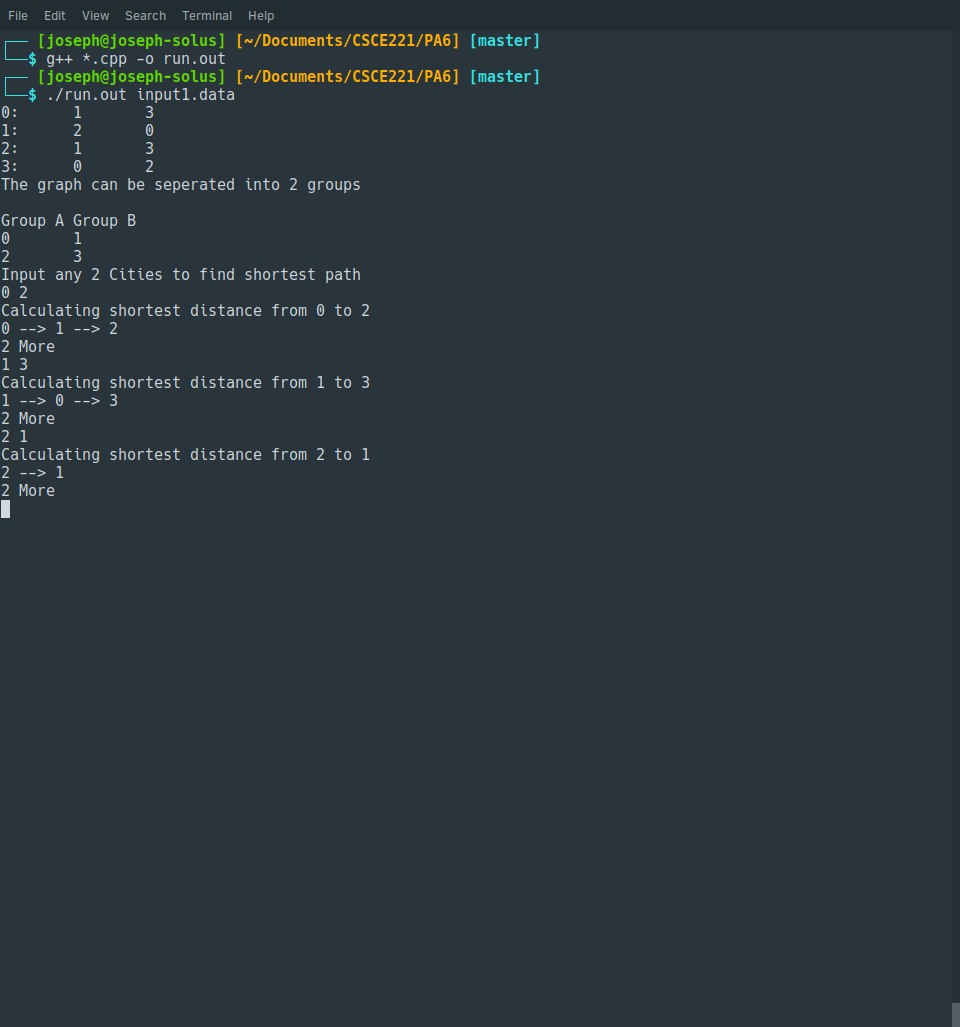
\includegraphics[scale=.4]{input01img.png}
  \end{center}
\end{figure}

With the following input, \\
5 6 \\
1 2 -1 \\
0 2 -1 \\
0 1 3 4 -1 \\
2 4 -1 \\
2 3 -1 \\
Results in the following output \\
\begin{figure}[h]
  \begin{center}
    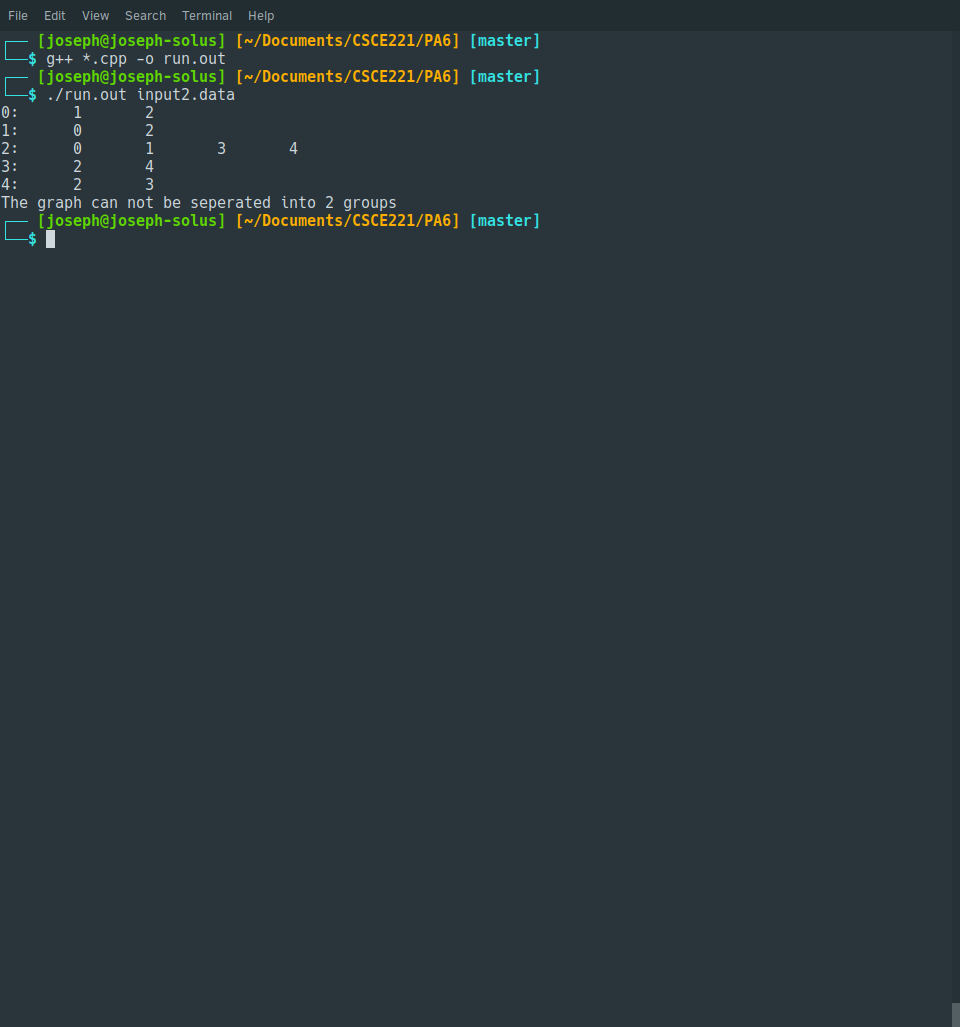
\includegraphics[scale=.4]{input2img.png}
  \end{center}
\end{figure}

With the following input, \\
7 6 \\
1 2 -1 \\
0 3 4 -1 \\
0 5 6 -1 \\
1 -1 \\
1 -1 \\
2 -1 \\
2 -1 \\
Results in the following output \\
\begin{figure}[h]
  \begin{center}
    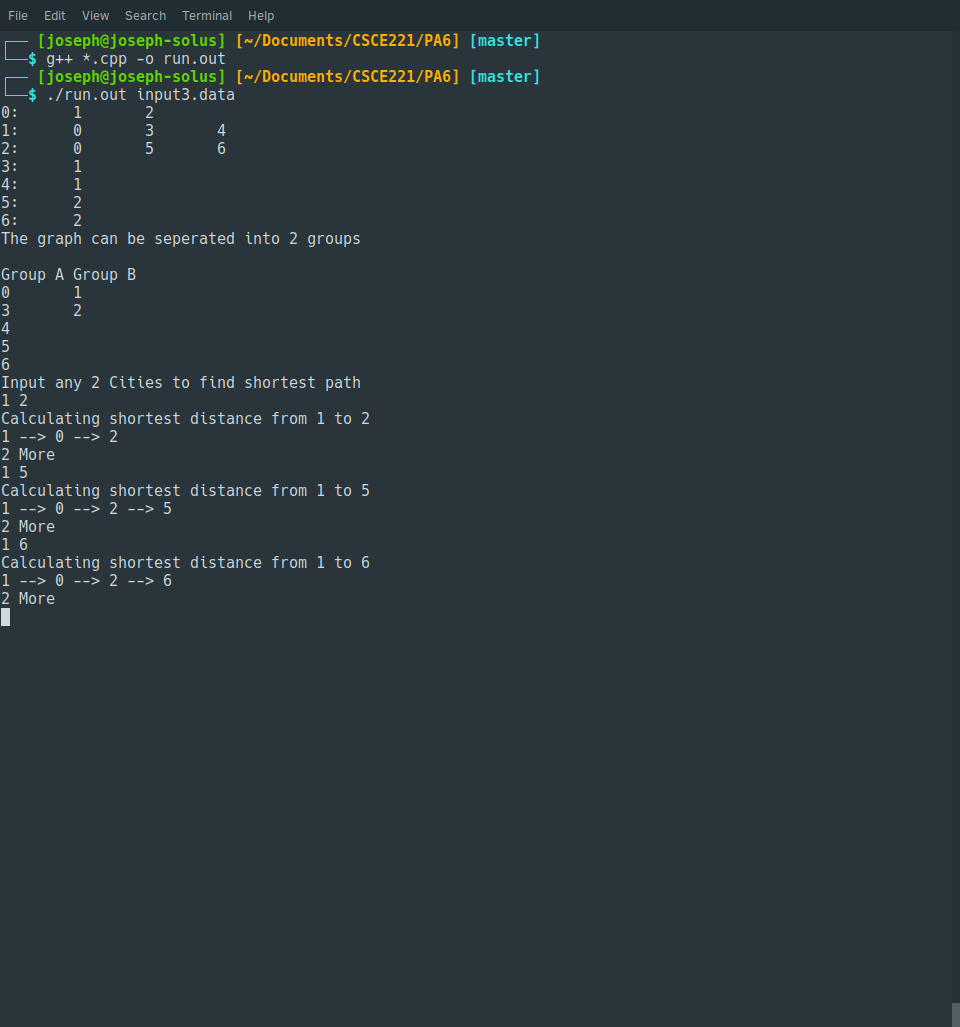
\includegraphics[scale=.4]{input3img.png}
  \end{center}
\end{figure}
\end{enumerate}

\end{document}
